% =========================================================
% Limit Superior and Limit Inferior
% File: notes-limsup-liminf.tex
% =========================================================

\subsection{Limit Superior and Limit Inferior}

% ---------------------------------------------------------
% Toolkit
% ---------------------------------------------------------
\begin{tcolorbox}[colback=gray!6, colframe=gray!40, arc=2pt,
  left=6pt, right=6pt, top=4pt, bottom=4pt,
  title={\small\textbf{Limsup Liminf — Quick Reference}},
  fonttitle=\small\bfseries]
\begin{tabular}{@{}p{0.28\textwidth}p{0.68\textwidth}@{}}
\textbf{Core items} & Key definitions/results introduced in this file.\\
\textbf{How to use} & Read the boxed items first; proofs and consequences follow.\\
\textbf{Dependencies} & Refer back to earlier sections as needed.\\
\end{tabular}
\end{tcolorbox}


% (Original local heading preserved)
\subsubsection{Limit Superior and Limit Inferior}

% ---------------------------------------------------------
\subsubsection{Basic Definitions}

\begin{tcolorbox}[colback=propbox, colframe=propborder, arc=2pt,
  left=6pt, right=6pt, top=4pt, bottom=4pt,
  title={\small\textbf{Definition (Tail supremum and infimum)}},
  fonttitle=\small\bfseries]
Let $(a_n)$ be a bounded real sequence. For each $n \in \mathbb{N}$ define
\[
s_n := \sup \{ a_k : k \ge n \},
\qquad
i_n := \inf \{ a_k : k \ge n \}.
\]
The sequences $(s_n)$ and $(i_n)$ are called the \emph{tail suprema} and 
\emph{tail infima} of $(a_n)$.
\end{tcolorbox}

\begin{theorem}[Monotonicity of tail suprema and infima]
Let $(x_n)$ be a real sequence and define
\[
s_n := \sup\{x_k : k\ge n\},
\qquad
i_n := \inf\{x_k : k\ge n\}.
\]
Then $(s_n)$ is decreasing and $(i_n)$ is increasing. In particular, each of $(s_n)$ and $(i_n)$
has a limit in $\mathbb{R}\cup\{\pm\infty\}$, and these limits are $\limsup x_n$ and $\liminf x_n$.
\end{theorem}

\begin{proof}
For each $n$, the tail set $\{x_k:k\ge n+1\}$ is a subset of the tail set $\{x_k:k\ge n\}$.
Therefore,
\[
s_{n+1}=\sup\{x_k:k\ge n+1\} \le \sup\{x_k:k\ge n\}=s_n,
\]
so $(s_n)$ is decreasing. Similarly,
\[
i_{n+1}=\inf\{x_k:k\ge n+1\} \ge \inf\{x_k:k\ge n\}=i_n,
\]
so $(i_n)$ is increasing.

A monotone real sequence always has a limit in the extended real line
$\mathbb{R}\cup\{\pm\infty\}$ (possibly infinite), so both $\lim s_n$ and $\lim i_n$ exist in that sense,
and by definition these are $\limsup x_n$ and $\liminf x_n$.
\end{proof}

\begin{tcolorbox}[colback=propbox, colframe=propborder, arc=2pt,
  left=6pt, right=6pt, top=4pt, bottom=4pt,
  title={\small\textbf{Definition (Limit superior and limit inferior)}},
  fonttitle=\small\bfseries]
Let $(a_n)$ be a bounded real sequence. The \emph{limit superior} and 
\emph{limit inferior} of $(a_n)$ are defined by
\[
\limsup_{n\to\infty} a_n := \lim_{n\to\infty} s_n,
\qquad
\liminf_{n\to\infty} a_n := \lim_{n\to\infty} i_n,
\]
where $s_n$ and $i_n$ are the tail supremum and tail infimum sequences.
\end{tcolorbox}

% (Original earlier definition preserved verbatim from source extract)
\begin{tcolorbox}[colback=propbox, colframe=propborder, arc=2pt,
  left=6pt, right=6pt, top=4pt, bottom=4pt,
  title={\small\textbf{Definition (Limit superior and limit inferior)}},
  fonttitle=\small\bfseries]
Let $(x_n)$ be a real sequence. Define
\[
s_n := \sup\{x_k : k\ge n\},
\qquad
i_n := \inf\{x_k : k\ge n\}.
\]
The \emph{limit superior} and \emph{limit inferior} of $(x_n)$ are
\[
\limsup_{n\to\infty} x_n := \lim_{n\to\infty} s_n,
\qquad
\liminf_{n\to\infty} x_n := \lim_{n\to\infty} i_n,
\]
provided these limits exist in $\mathbb{R}\cup\{\pm\infty\}$.
\end{tcolorbox}

% ---------------------------------------------------------
\subsubsection{Main Theorems}

\begin{theorem}[Equivalent formulation as inf-sup]
For any bounded sequence $(a_n)$,
\[
\limsup_{n\to\infty} a_n = \inf_{n \ge 1} \sup_{k \ge n} a_k,
\qquad
\liminf_{n\to\infty} a_n = \sup_{n \ge 1} \inf_{k \ge n} a_k.
\]
\end{theorem}

\begin{proof}
Let $s_n = \sup\{a_k : k \ge n\}$. Since $(s_n)$ is decreasing and bounded below,
$\lim_{n\to\infty} s_n = \inf_{n \ge 1} s_n = \inf_{n \ge 1} \sup_{k \ge n} a_k$.
The $\liminf$ case is analogous.
\end{proof}

\begin{theorem}[Equivalent characterizations]
Let $(a_n)$ be bounded and let $L = \limsup_{n\to\infty} a_n$. Then:

\begin{enumerate}
\item $a_n > L - \varepsilon$ for infinitely many $n$ for every $\varepsilon>0$.
\item For every $\varepsilon>0$, $a_n < L + \varepsilon$ for all sufficiently large $n$.
\end{enumerate}

Similarly, if $l = \liminf_{n\to\infty} a_n$, then:

\begin{enumerate}
\item $a_n < l + \varepsilon$ for infinitely many $n$ for every $\varepsilon>0$.
\item For every $\varepsilon>0$, $a_n > l - \varepsilon$ for all sufficiently large $n$.
\end{enumerate}
\end{theorem}

\begin{proof}
We prove the characterization for $\limsup$; the $\liminf$ case follows by symmetry.

Let $s_n = \sup\{a_k : k \ge n\}$, so $L = \lim_{n\to\infty} s_n$.

\textbf{Property (1):} Fix $\varepsilon > 0$. We must show infinitely many $a_n > L - \varepsilon$.
Suppose not; then $a_n \le L - \varepsilon$ for all $n \ge N$ for some $N$.
This means $s_N = \sup\{a_k : k \ge N\} \le L - \varepsilon$.
Since $(s_n)$ is decreasing, $s_n \le s_N \le L - \varepsilon$ for all $n \ge N$.
Thus $L = \lim s_n \le L - \varepsilon$, a contradiction.

\textbf{Property (2):} Fix $\varepsilon > 0$. Since $s_n \to L$, there exists $N$ such that
$s_n < L + \varepsilon$ for all $n \ge N$.
For any $k \ge N$, we have $a_k \le s_N < L + \varepsilon$.
Thus $a_n < L + \varepsilon$ for all $n \ge N$.

\textbf{Uniqueness:} Suppose $L'$ also satisfies properties (1) and (2). 
If $L' > L$, choose $\varepsilon = (L' - L)/2$. 
By property (2) for $L$, eventually $a_n < L + \varepsilon = L' - \varepsilon$.
But property (1) for $L'$ requires infinitely many $a_n > L' - \varepsilon$, contradiction.
Similarly $L' < L$ leads to contradiction. Thus $L' = L$.
\end{proof}

\begin{theorem}[Basic inequalities]
Let $(a_n)$ be bounded. Then
\[
\inf_{n\in\mathbb{N}} a_n
\;\le\;
\liminf_{n\to\infty} a_n
\;\le\;
\limsup_{n\to\infty} a_n
\;\le\;
\sup_{n\in\mathbb{N}} a_n.
\]
\end{theorem}

\begin{theorem}[Sign symmetry]
For any bounded sequence $(a_n)$,
\[
\limsup_{n\to\infty} (-a_n)
=
-\,\liminf_{n\to\infty} a_n,
\qquad
\liminf_{n\to\infty} (-a_n)
=
-\,\limsup_{n\to\infty} a_n.
\]
\end{theorem}

\begin{theorem}[Order preservation]
Let $(a_n)$ and $(b_n)$ be bounded sequences. If
\[
a_n \le b_n \quad \text{for all } n,
\]
then
\[
\liminf_{n\to\infty} a_n
\;\le\;
\liminf_{n\to\infty} b_n,
\qquad
\limsup_{n\to\infty} a_n
\;\le\;
\limsup_{n\to\infty} b_n.
\]
\end{theorem}

\begin{theorem}[Subadditivity of $\limsup$]
Let $(a_n)$ and $(b_n)$ be bounded sequences. Then
\[
\limsup_{n\to\infty} (a_n + b_n)
\;\le\;
\limsup_{n\to\infty} a_n
+
\limsup_{n\to\infty} b_n.
\]
\end{theorem}

\begin{proof}
Let $s_n^a = \sup\{a_k : k \ge n\}$, $s_n^b = \sup\{b_k : k \ge n\}$, and 
$s_n^{a+b} = \sup\{a_k + b_k : k \ge n\}$.

For any $k \ge n$, we have $a_k \le s_n^a$ and $b_k \le s_n^b$, so
$a_k + b_k \le s_n^a + s_n^b$.
Taking the supremum over $k \ge n$ gives $s_n^{a+b} \le s_n^a + s_n^b$.

Taking the limit as $n \to \infty$:
\[
\limsup(a_n + b_n) = \lim_{n\to\infty} s_n^{a+b} 
\le \lim_{n\to\infty}(s_n^a + s_n^b)
= \limsup a_n + \limsup b_n. \qedhere
\]
\end{proof}

\begin{theorem}[Superadditivity of $\liminf$]
Let $(a_n)$ and $(b_n)$ be bounded sequences. Then
\[
\liminf_{n\to\infty} a_n
+
\liminf_{n\to\infty} b_n
\;\le\;
\liminf_{n\to\infty} (a_n + b_n).
\]
\end{theorem}

\begin{proof}
Apply sign symmetry and subadditivity:
\begin{align*}
\liminf a_n + \liminf b_n 
&= -\limsup(-a_n) - \limsup(-b_n) \\
&= -\bigl(\limsup(-a_n) + \limsup(-b_n)\bigr) \\
&\le -\limsup\bigl((-a_n) + (-b_n)\bigr) \\
&= -\limsup(-(a_n + b_n)) \\
&= \liminf(a_n + b_n). \qedhere
\end{align*}
\end{proof}

\begin{theorem}[Equality when one sequence converges]
Suppose $(a_n)$ converges to $a$ and $(b_n)$ is bounded. Then
\[
\limsup_{n\to\infty}(a_n + b_n) = a + \limsup_{n\to\infty} b_n,
\]
\[
\liminf_{n\to\infty}(a_n + b_n) = a + \liminf_{n\to\infty} b_n.
\]
\end{theorem}

\begin{proof}
We prove the $\limsup$ case. By subadditivity applied twice:
\[
\limsup(a_n + b_n) \le \limsup a_n + \limsup b_n = a + \limsup b_n,
\]
and
\[
\limsup b_n = \limsup\bigl((a_n + b_n) + (-a_n)\bigr) 
\le \limsup(a_n + b_n) + \limsup(-a_n)
= \limsup(a_n + b_n) - a.
\]
Rearranging gives $a + \limsup b_n \le \limsup(a_n + b_n)$.
The $\liminf$ case follows by sign symmetry.
\end{proof}

\begin{theorem}[Addition law for convergent sequences]
Suppose $(a_n)$ and $(b_n)$ are bounded sequences such that
$a_n \to a$ and $b_n \to b$. Then

\[
\limsup (a_n + b_n) = a + b
\qquad \text{and} \qquad
\liminf (a_n + b_n) = a + b.
\]
\end{theorem}

\begin{proof}
Since $a_n \to a$ and $b_n \to b$, we have
$\limsup a_n = \liminf a_n = a$
and
$\limsup b_n = \liminf b_n = b$.
Using subadditivity and symmetry yields the result.
\end{proof}

\begin{theorem}[Scalar multiplication]
Let $(a_n)$ be a bounded sequence and $c \in \mathbb{R}$. Then:
\begin{enumerate}
\item If $c > 0$:
\[
\limsup_{n\to\infty}(c \cdot a_n) = c \cdot \limsup_{n\to\infty} a_n,
\qquad
\liminf_{n\to\infty}(c \cdot a_n) = c \cdot \liminf_{n\to\infty} a_n.
\]
\item If $c < 0$:
\[
\limsup_{n\to\infty}(c \cdot a_n) = c \cdot \liminf_{n\to\infty} a_n,
\qquad
\liminf_{n\to\infty}(c \cdot a_n) = c \cdot \limsup_{n\to\infty} a_n.
\]
\item If $c = 0$: $\limsup(c \cdot a_n) = \liminf(c \cdot a_n) = 0$.
\end{enumerate}
\end{theorem}

\begin{proof}
For $c > 0$: Since $\sup(cA) = c \sup(A)$ for any bounded set $A$ and $c > 0$,
\[
\sup\{c \cdot a_k : k \ge n\} = c \cdot \sup\{a_k : k \ge n\}.
\]
Taking limits gives the result. The $\liminf$ case is analogous.

For $c < 0$: Write $c = -|c|$ and use sign symmetry:
\[
\limsup(c \cdot a_n) = \limsup(-|c| \cdot a_n) = -\liminf(|c| \cdot a_n) = -|c| \cdot \liminf a_n = c \cdot \liminf a_n.
\]
The second identity follows similarly.
\end{proof}

\begin{theorem}[Product inequality for nonnegative sequences]
Let $(a_n)$ and $(b_n)$ be bounded sequences with $a_n \ge 0$ and $b_n \ge 0$ for all $n$. Then
\[
\limsup_{n\to\infty}(a_n b_n) \le \bigl(\limsup_{n\to\infty} a_n\bigr)\bigl(\limsup_{n\to\infty} b_n\bigr).
\]
\end{theorem}

\begin{proof}
Let $L = \limsup a_n$ and $M = \limsup b_n$. For any $\varepsilon > 0$, there exists $N$ such that
$a_n < L + \varepsilon$ and $b_n < M + \varepsilon$ for all $n \ge N$.
Thus for $n \ge N$:
\[
a_n b_n < (L + \varepsilon)(M + \varepsilon).
\]
Taking $\limsup$ and then $\varepsilon \to 0$ gives the result.
\end{proof}

\begin{theorem}[Characterization via subsequences]
Let $(a_n)$ be bounded. Then
\[
\limsup_{n\to\infty} a_n
=
\sup \{ \ell : \ell \text{ is a subsequential limit of } (a_n) \},
\]
and
\[
\liminf_{n\to\infty} a_n
=
\inf \{ \ell : \ell \text{ is a subsequential limit of } (a_n) \}.
\]
\end{theorem}

\begin{proof}
Let $L = \limsup a_n$ and let $S$ denote the set of all subsequential limits of $(a_n)$.
We show $L = \sup S$.

\textbf{Step 1:} $L \in S$ (so $L \le \sup S$ is immediate once we show $L$ is achieved).
By the $\varepsilon$-characterization, for each $k \in \mathbb{N}$, there exists $n_k$ with
$a_{n_k} > L - 1/k$. We can choose $n_k$ strictly increasing.
Also, $a_{n_k} < L + 1/k$ for large $k$ by property (2).
Thus $|a_{n_k} - L| < 1/k$ for large $k$, so $a_{n_k} \to L$. Hence $L \in S$.

\textbf{Step 2:} $L \ge \sup S$.
Suppose $(a_{n_k})$ is a subsequence converging to some $\ell$.
By property (2) of the $\varepsilon$-characterization, for any $\varepsilon > 0$,
$a_n < L + \varepsilon$ for all sufficiently large $n$.
Thus $a_{n_k} < L + \varepsilon$ for large $k$, so $\ell \le L + \varepsilon$.
Since $\varepsilon$ was arbitrary, $\ell \le L$. This holds for all $\ell \in S$, so $\sup S \le L$.

The $\liminf$ case follows by applying the above to $(-a_n)$ and using sign symmetry.
\end{proof}

\begin{theorem}[Extremal subsequences]
Let $(a_n)$ be bounded. Then there exist subsequences
$(a_{n_k})$ and $(a_{m_k})$ such that

\[
a_{n_k} \to \limsup_{n\to\infty} a_n,
\qquad
a_{m_k} \to \liminf_{n\to\infty} a_n.
\]
\end{theorem}

\begin{proof}
Let $L=\limsup a_n$. By the characterization theorem,
for each $k$ there exists $n_k$ such that
\[
a_{n_k} > L - \frac{1}{k}.
\]
Choosing $n_k$ strictly increasing produces a subsequence
converging to $L$. The argument for $\liminf$ is similar.
\end{proof}

\begin{theorem}[Convergence criterion]
A bounded sequence $(a_n)$ converges if and only if
\[
\limsup_{n\to\infty} a_n
=
\liminf_{n\to\infty} a_n.
\]
In this case,
\[
\lim_{n\to\infty} a_n
=
\limsup_{n\to\infty} a_n
=
\liminf_{n\to\infty} a_n.
\]
\end{theorem}

% ---------------------------------------------------------
% Examples / Figures (kept verbatim; placed where they support the theory)
% ---------------------------------------------------------

\begin{tcolorbox}[colback=propbox, colframe=propborder, arc=2pt,
  left=6pt, right=6pt, top=4pt, bottom=4pt,
  title={\small\textbf{Example (Strict inequality in subadditivity)}},
  fonttitle=\small\bfseries]
Let $a_n = (-1)^n$ and $b_n = (-1)^{n+1} = -a_n$. Then $a_n + b_n = 0$ for all $n$, so
\[
\limsup(a_n + b_n) = 0.
\]
However, $\limsup a_n = 1$ and $\limsup b_n = 1$, so
\[
\limsup a_n + \limsup b_n = 2.
\]
Thus the inequality $\limsup(a_n + b_n) \le \limsup a_n + \limsup b_n$ can be strict.
\end{tcolorbox}

\begin{tcolorbox}[colback=propbox, colframe=propborder, arc=2pt,
  left=6pt, right=6pt, top=4pt, bottom=4pt,
  title={\small\textbf{Example (Strict inequality in product rule)}},
  fonttitle=\small\bfseries]
Let $a_n = \frac{1 + (-1)^n}{2}$ (alternates $0, 1, 0, 1, \ldots$) and 
$b_n = \frac{1 + (-1)^{n+1}}{2}$ (alternates $1, 0, 1, 0, \ldots$).
Then $a_n b_n = 0$ for all $n$, so $\limsup(a_n b_n) = 0$.
But $\limsup a_n = 1$ and $\limsup b_n = 1$, so the product of $\limsup$'s is $1$.
\end{tcolorbox}

% Requires:
% \usepackage{tikz}
% \usetikzlibrary{calc}

\begin{figure}[h]
\centering
\begin{tikzpicture}[x=0.55cm,y=0.95cm, line cap=round, line join=round]

% -----------------------------
% Parameters
% -----------------------------
\def\N{52}           % number of terms shown
\def\dotR{1.4pt}     % dot radius

\def\Linf{0.55}      % illustrative lim inf level
\def\Lsup{1.65}      % illustrative lim sup level
\pgfmathsetmacro{\mid}{0.5*(\Linf+\Lsup)}
\pgfmathsetmacro{\A}{0.5*(\Lsup-\Linf)} % half-width of the band

% Room so labels/dots never clip
\useasboundingbox (-1.2,-0.3) rectangle (\N+2.3,2.25);

% -----------------------------
% Axis
% -----------------------------
\draw[->,thick] (0,0) -- (\N+2,0) node[below] {$n$};

% -----------------------------
% Band FIRST (so dots appear on top)
% -----------------------------
\fill[red!10] (0,\Linf) rectangle (\N+1.5,\Lsup);

\draw[red!70, dashed, thick] (0,\Linf) -- (\N+1.5,\Linf);
\draw[red!70, dashed, thick] (0,\Lsup) -- (\N+1.5,\Lsup);

\node[black!70, anchor=west] at (1.0,\Linf+0.06) {$\liminf_{n\to\infty} a_n$};
\node[black!70, anchor=west] at (1.0,\Lsup+0.06) {$\limsup_{n\to\infty} a_n$};

% ---------------------------------------
% Oscillation with transient (Option B)
%   - persistent oscillation => limsup=Lsup, liminf=Linf
%   - transient dies out => points eventually stay in the band
% ---------------------------------------

% transient strength / decay rate (tune these)
\def\T{1.05}      % transient amplitude (makes early points outside band)
\def\k{0.22}      % decay rate (bigger => faster decay)

% Dots at integer n (this is the actual sequence (a_n))
\foreach \n in {1,...,\N} {%
  \pgfmathsetmacro{\yy}{
    \mid
    + \A*sin(90*\n)
    + \T*exp(-\k*\n)*sin(35*\n)
  }%
  \fill[black] (\n,\yy) circle (\dotR);%
}

% Dots on top
\foreach \n in {1,...,\N} {%
  \pgfmathsetmacro{\yy}{\mid + (2.2*exp(-0.08*\n))*sin(0.55*\n r)}%
  \fill[black] (\n,\yy) circle (\dotR);%
}

\end{tikzpicture}
\caption{Illustration of \(\liminf a_n\) and \(\limsup a_n\): the oscillation persists, but the transient dies out so points eventually lie within the band.}
\end{figure}

% ---------------------------------------------------------
\subsubsection{Consequences}

The logical implication of this entire section is:

\begin{itemize}
\item Tail suprema/infima are monotone (hence have extended real limits).
\item $\limsup$ and $\liminf$ can be characterized in multiple equivalent ways:
  as limits of tail extrema, as inf--sup / sup--inf, and via $\varepsilon$-style
  ``infinitely often'' / ``eventually'' conditions.
\item $\limsup$ and $\liminf$ behave functorially with order, addition, and scalar multiplication
  (with inequalities in general, and equalities under convergence hypotheses).
\item A bounded sequence converges exactly when its two extreme limiting behaviors coincide:
\[
\limsup a_n = \liminf a_n \Longleftrightarrow a_n \text{ converges},
\]
and then all three values equal the common limit.
\end{itemize}

\begin{remark}
The limit superior and limit inferior capture the largest and smallest
possible limiting behavior of a bounded sequence.

The number $\limsup a_n$ is the largest subsequential limit,
while $\liminf a_n$ is the smallest subsequential limit.
A sequence converges precisely when these two extreme behaviors coincide.
\end{remark}

\begin{remark}[Logical Structure]
A clean dependency chain is:
\[
\text{Tail sup/inf}
\Rightarrow
\text{Monotonicity of tail sup/inf}
\Rightarrow
\limsup/\liminf \text{ (definitions)}
\Rightarrow
\text{Characterizations and algebraic laws}
\Rightarrow
\text{Subsequence interpretation}
\Rightarrow
\text{Convergence criterion}.
\]
\end{remark}

\begin{remark}[From limit superior and inferior to series]
The machinery of limit superior and inferior developed in this section
is not merely a tool for studying individual sequences --- it is the
natural language for convergence tests on infinite series.

Recall that an infinite series
\[
\sum_{n=1}^{\infty} a_n
\]
is defined as the limit of its sequence of partial sums
\[
S_N := \sum_{n=1}^{N} a_n.
\]
Convergence of the series is therefore convergence of the sequence
$(S_N)$, and all prior theory applies directly.

The connection to limsup and liminf is concrete:
\begin{itemize}
  \item The \emph{Root Test} determines convergence via
        $\limsup_{n\to\infty} |a_n|^{1/n}$, which exists for any
        sequence and captures the worst-case exponential growth rate
        of the terms.
  \item The \emph{Ratio Test} uses
        $\limsup_{n\to\infty} |a_{n+1}/a_n|$ and
        $\liminf_{n\to\infty} |a_{n+1}/a_n|$ to give sharp
        convergence and divergence conditions.
  \item The \emph{Cauchy condensation test} and comparison arguments
        rely on tail behavior, which is precisely what limsup and
        liminf measure.
\end{itemize}

In each case, the test reduces a question about a series to a question
about the limiting behavior of a sequence of real numbers --- exactly
the setting limsup and liminf were built for.

The series section that follows should therefore be read as an
application of the full sequence theory developed so far, with
limsup and liminf as the central technical tool.
\end{remark}
